\documentclass[12pt,letter]{article}
\usepackage[moduleName=S-SMP(ADSR)]{KautenjaDSP}
\begin{document}
\titlePage{img/Logo}{img/Module}{img/KautenjaDSP}

% -------------------
% MARK: Overview
% -------------------

\section{Overview}

\begin{figure}[!htp]
\centering
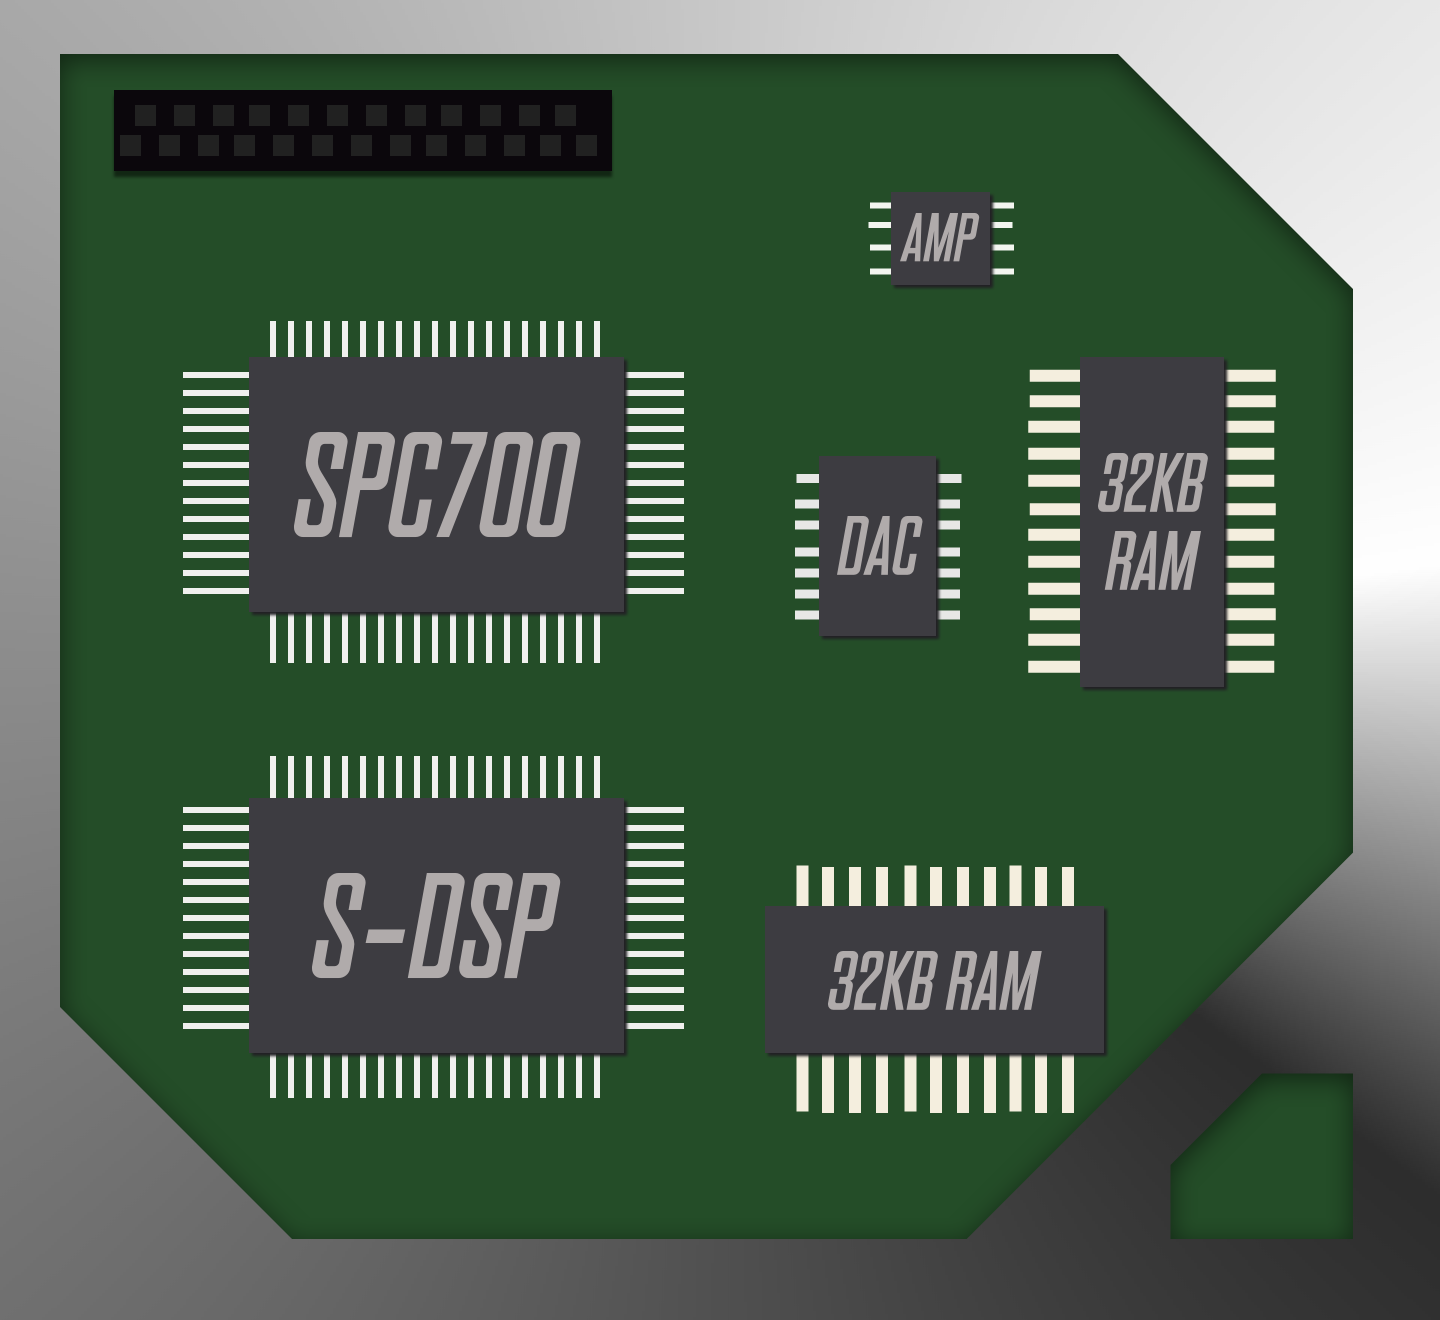
\includegraphics[width=0.5\textwidth]{img/S-SMP-Chip}
\caption{The S-SMP module from the SNES. The S-SMP included two discrete microprocessors: the SPC700, and the S-DSP. The SPC700 performed primary computation, while the S-DSP performed DSP specific computations, like BRR decoding, sample playback, applying the echo effect, mixing levels, etc. The SPC700 and S-DSP shared $64KB$ of total RAM that was used for BRR sample data and the echo buffer. The digital audio is decoded back to an analog signal by a 16-bit DAC and amplified using an Op-Amp. Before digital-to-analog conversion, the output audio is low-pass filtered by a Gaussian filter that gives the S-SMP chip a distinctive sound.}
\end{figure}

\clearpage

S-SMP(ADSR) is a Eurorack module that emulates the ADSR envelope generator from the S-SMP sound chip on the Super Nintendo Entertainment System (SNES). The ADSR on the SNES has (1) a linear attack stage, followed by (2) a non-linear decay stage that falls to a (3) sustain level that maintains for a (4) sustain rate or until key-off. On key-off the envelope quickly releases to zero in a way that produces minimal popping and clicks.

S-SMP(ADSR) provides the key features of the ADSR of the S-SMP chip,
namely,
\begin{itemize}
  \item \textbf{$32KHz$ Sample Rate:} The S-SMP was designed to run at $32kHz$, so the audio inputs and outputs of the module are locked to $32kHz$.
  \item \textbf{Stereo ADSR:} Dual envelope generators for stereo effects, modulation, or self modulation.
  \item \textbf{Bipolar Level Control:} Control the total height of the envelope (i.e., the point the attack stage stops at), including the ability to polarize the envelope into negative voltages.
\end{itemize}

% -------------------
% MARK: Panel Layout
% -------------------

\clearpage
\section{Panel Layout}

\begin{figure}[!htp]
\centering
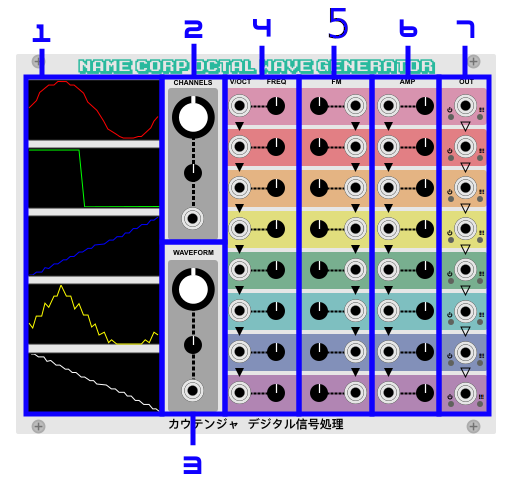
\includegraphics{img/Interface}
\end{figure}

\clearpage
\begin{enumerate}
  \item TODO
\end{enumerate}

% -------------------
% MARK: References
% -------------------

\clearpage
\renewcommand\refname{References}
\nocite{*}
\bibliographystyle{apalike}
\bibliography{references}

\end{document}
